\documentclass{beamer}

\usepackage[utf8]{inputenc}
\usepackage[T1]{fontenc}
\usepackage{setspace}
\usepackage{color}
\usepackage{listings}
\usepackage{zi4}
\usepackage{tikz}

\usetheme{Frankfurt}

\lstset{basicstyle=\ttfamily,breaklines=true}

\definecolor{javared}{rgb}{0.6,0,0} % for strings
\definecolor{javagreen}{rgb}{0.25,0.5,0.35} % comments
\definecolor{javapurple}{rgb}{0.5,0,0.35} % keywords
\definecolor{javadocblue}{rgb}{0.25,0.35,0.75} % javadoc
 
\lstset{language=Java,
basicstyle=\footnotesize\ttfamily,
keywordstyle=\color{javapurple}\bfseries,
stringstyle=\color{javared},
commentstyle=\color{javagreen},
morecomment=[s][\color{javadocblue}]{/**}{*/},
%numbers=left,
%numberstyle=\tiny\color{black},
%stepnumber=1,
%numbersep=10pt,
tabsize=4,
showspaces=false,
showstringspaces=false}


\lstdefinelanguage{Bytecode}{
  keywords={GETSTATIC, INVOKEVIRTUAL, LDC, RETURN},
  keywordstyle=\color{black}\bfseries,
  identifierstyle=\color{black},
  sensitive=false,
  comment=[l]{//},
  morecomment=[s]{/*}{*/},
  commentstyle=\color{purple}\ttfamily,
  stringstyle=\color{red}\ttfamily,
  morestring=[b]',
  morestring=[b]",
  basicstyle=\footnotesize\ttfamily
}

\begin{document}

\title[Optimization]
{Optimizing String manipulation performance}
\author{Markus Wondrak}
\institute
{
  Institute of Computer Science\\
  Johann Wolfgang von Goethe Universität, Frankfurt am Main
}

\frame{\titlepage}

\begin{frame}
  \frametitle{Table of Contents}
  \tableofcontents
\end{frame}

\section{Motivation}  

\begin{frame}[fragile]

  \frametitle{Example}
  \framesubtitle{The "normal" way}

  \begin{lstlisting}[language=Java]
String result = "";

for (int i = 0; i < line.length(); i += 2) {
  result += line.substring(i, i + 1);
}

return result;
  \end{lstlisting}%
\end{frame}


\begin{frame}[fragile]
  \frametitle{Example}
  \framesubtitle{The optimized way}
  \begin{lstlisting}[language=Java]
SubstringString lineOpt = new SubstringString(line);
  
StringListBuilder builder = new StringListBuilder();

for (int i = 0; i < line.length(); i+=2) {
  builder.append(lineOpt.substring(i, i + 1));
}

return builder.toString();
  \end{lstlisting}%
\end{frame}

\begin{frame}

   \frametitle{What is the difference}

\end{frame}

\begin{frame}
  \frametitle{Measurement}

\end{frame}

\begin{frame}
  \frametitle{Additional goals}
  \begin{itemize}
    \item Should be applicable to to already compiled programs aswell
  
  \end{itemize}
\end{frame}

\section{Bytecode}

\begin{frame}
   \frametitle{Bytecode}
   \begin{itemize}
      \item What the JVM actual executes (platform independence)
      \item Assembly language like 
      \item Stack-based and imperative
   \end{itemize}    
\end{frame}


\begin{frame}[fragile]
   \frametitle{Bytecode}
   Java:
   \begin{lstlisting}[language=Java]
System.out.println("Hallo World!");
  \end{lstlisting}%
  Bytecode:
  \begin{lstlisting}[language=Bytecode]
GETSTATIC java/lang/System.out : Ljava/io/PrintStream;
LDC "Hallo World!"
INVOKEVIRTUAL java/io/PrintStream.println (Ljava/lang/String;)V
RETURN
  \end{lstlisting}  
\end{frame}

\section{WALA}

\begin{frame}
   \frametitle{WALA}
   \begin{itemize}
      \item Watson Library of Analysis (IBM)
      
   \end{itemize}

\end{frame}

\begin{frame}
   \frametitle{Intermediate Representation}
   
   
\end{frame}

\section{Analysis}

\begin{frame}
   \frametitle{Naming}
   a variable in the IR, has exactly one definition and n uses
\end{frame}

\begin{frame}
   \frametitle{example graph}
   \begin{center}

   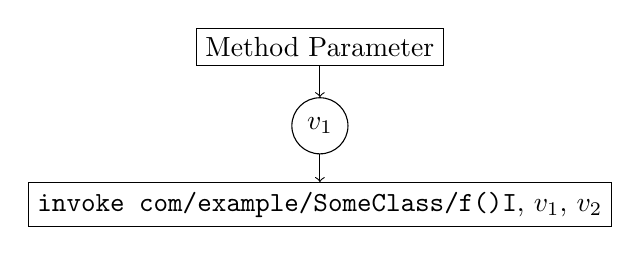
\begin{tikzpicture} 
    \node[draw,rectangle] (defv1) {Method Parameter};
    \node[draw,circle, below of=defv1] (v1) {$v_1$};
    \node[draw,rectangle, below of=v1] (invoke) {\texttt{invoke com/example/SomeClass/f()I}, $v_1$, $v_2$};
    
    \draw[->] (defv1) to (v1);
    \draw[->] (v1) to (invoke);
   \end{tikzpicture}
   \end{center}
\end{frame}


\end{document}